\documentclass[11pt, english]{article}
\usepackage{graphicx}
\usepackage{float}
\title{ Project 2 }
\date{}
\author{Abhinav Narain}
\begin{document}
\maketitle
\pagebreak
\section{Question 1: Benchmarks: Shannon limit and QPSK limit}
\begin{figure}[H]
    \centering
    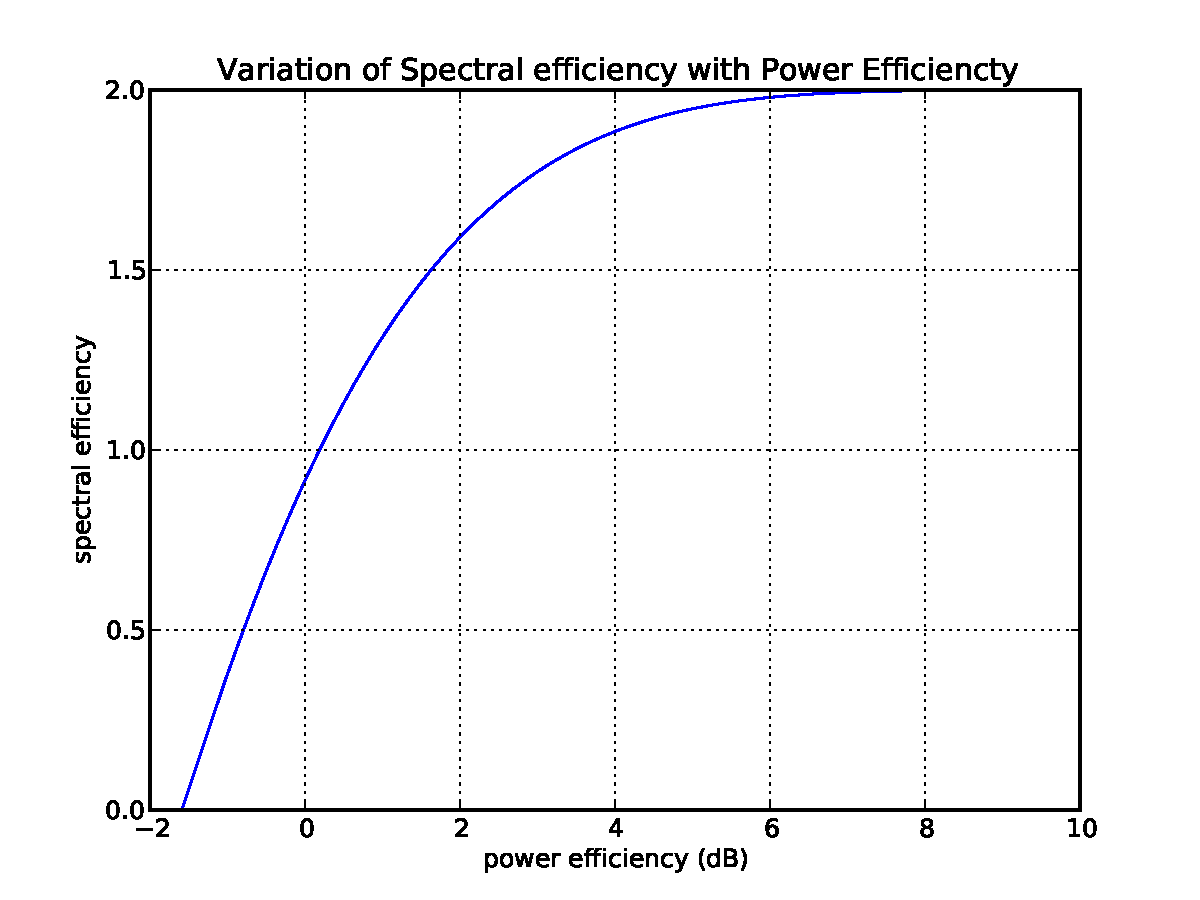
\includegraphics[width=.8\textwidth]{real_limit.pdf}
    \caption{plot using the fundamental equation}
    \label{rl}
\end{figure}
\begin{figure}[H]
    \centering
    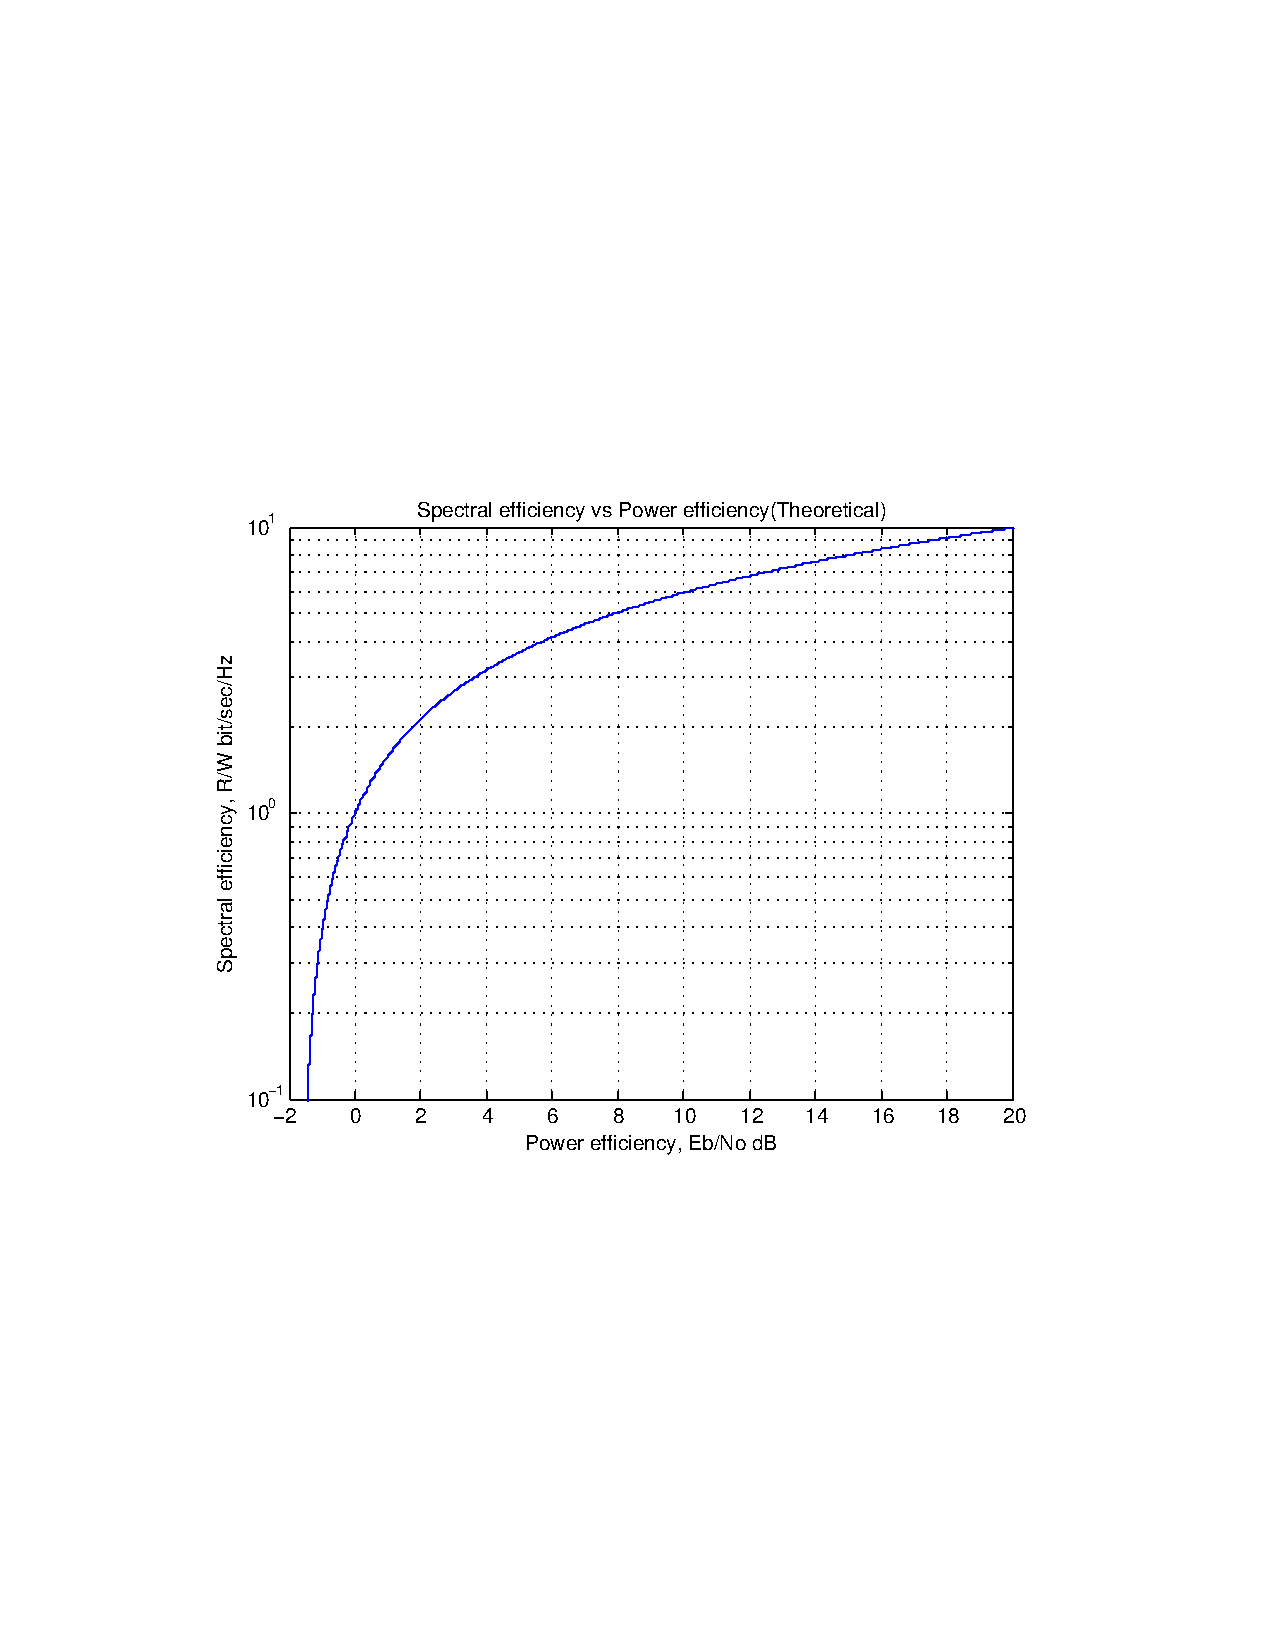
\includegraphics[width=.8\textwidth]{theoretical_limit.pdf}
    \caption{plot of Theoretical function}
    \label{th1}
\end{figure}

\section{Question 2: Uncoded QPSK}
\begin{figure}[H]
    \centering
    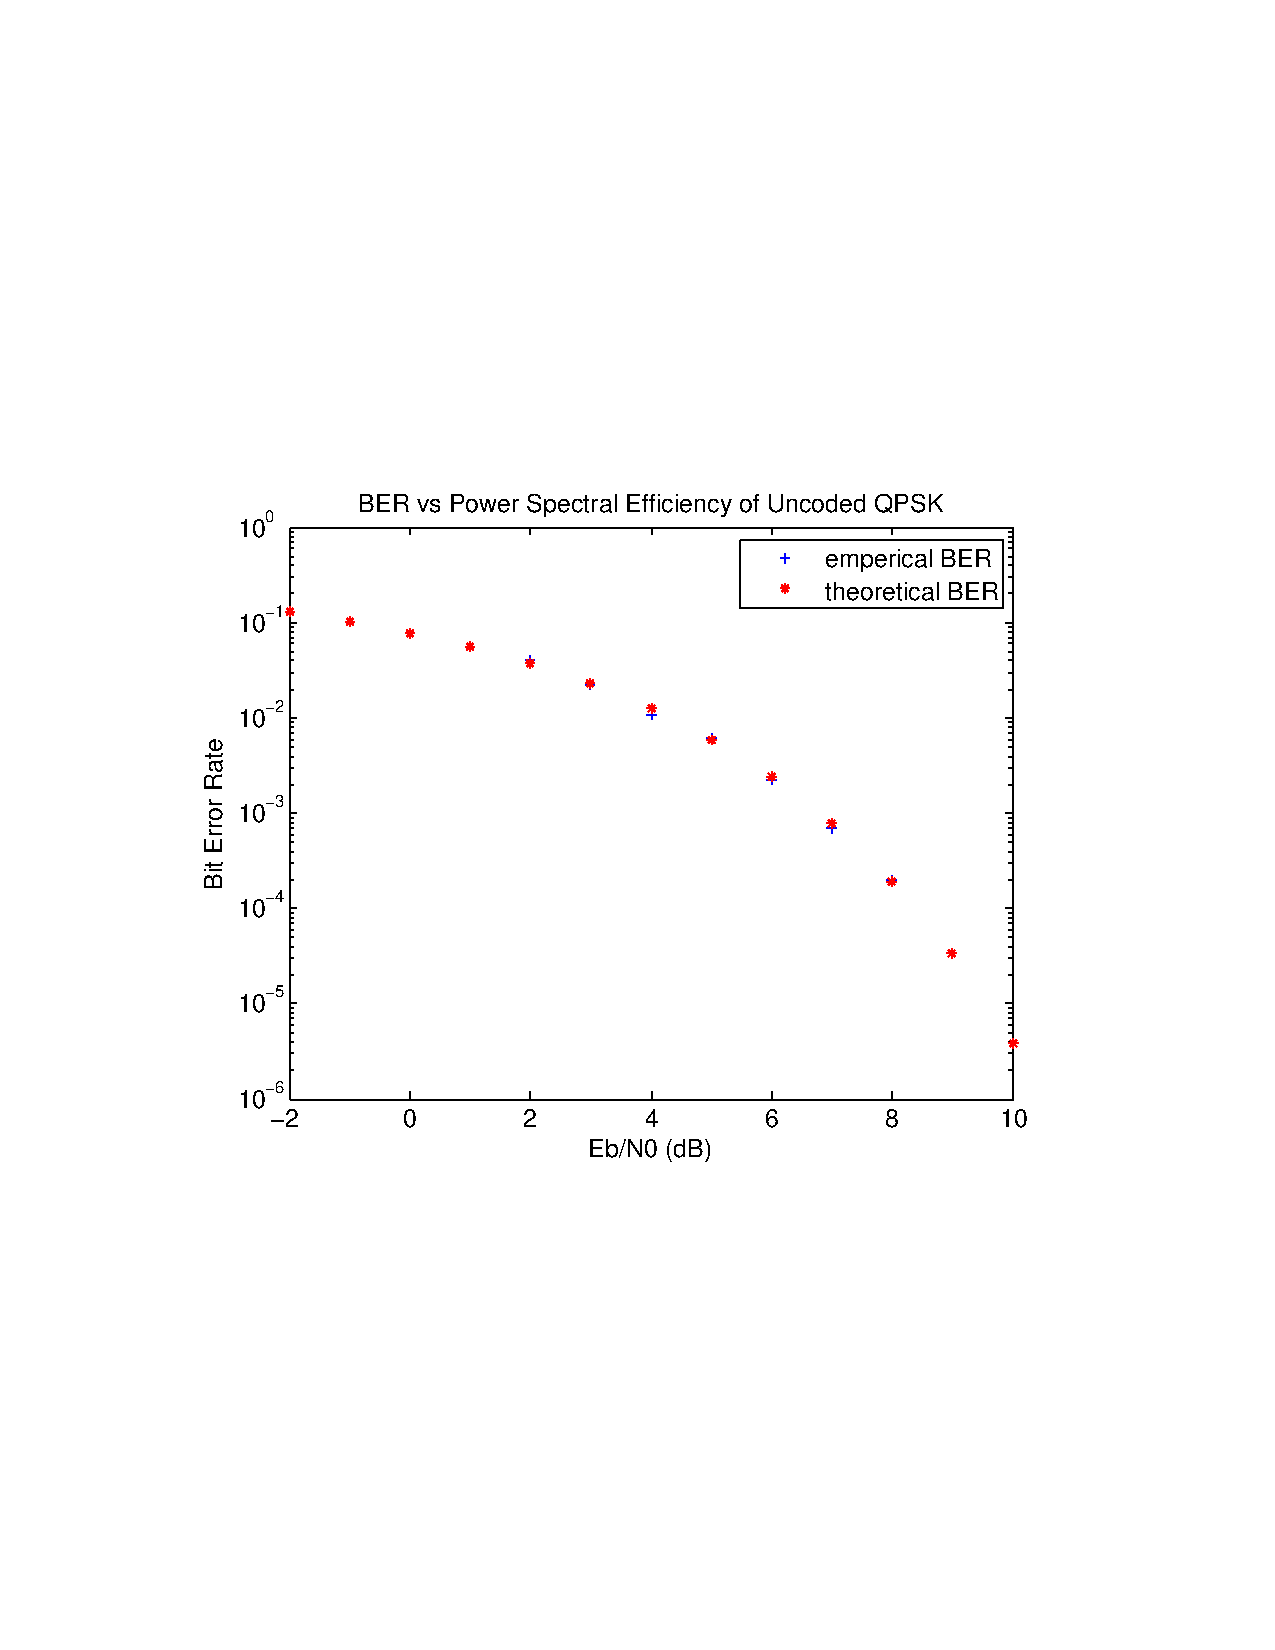
\includegraphics[width=.8\textwidth]{uncoded_qpsk.pdf}
    \caption{plot of Uncoded QPSK for }
    \label{th1}
\end{figure}

\section{Question 3: Repetition Codes}
\begin{figure}[H]
    \centering
    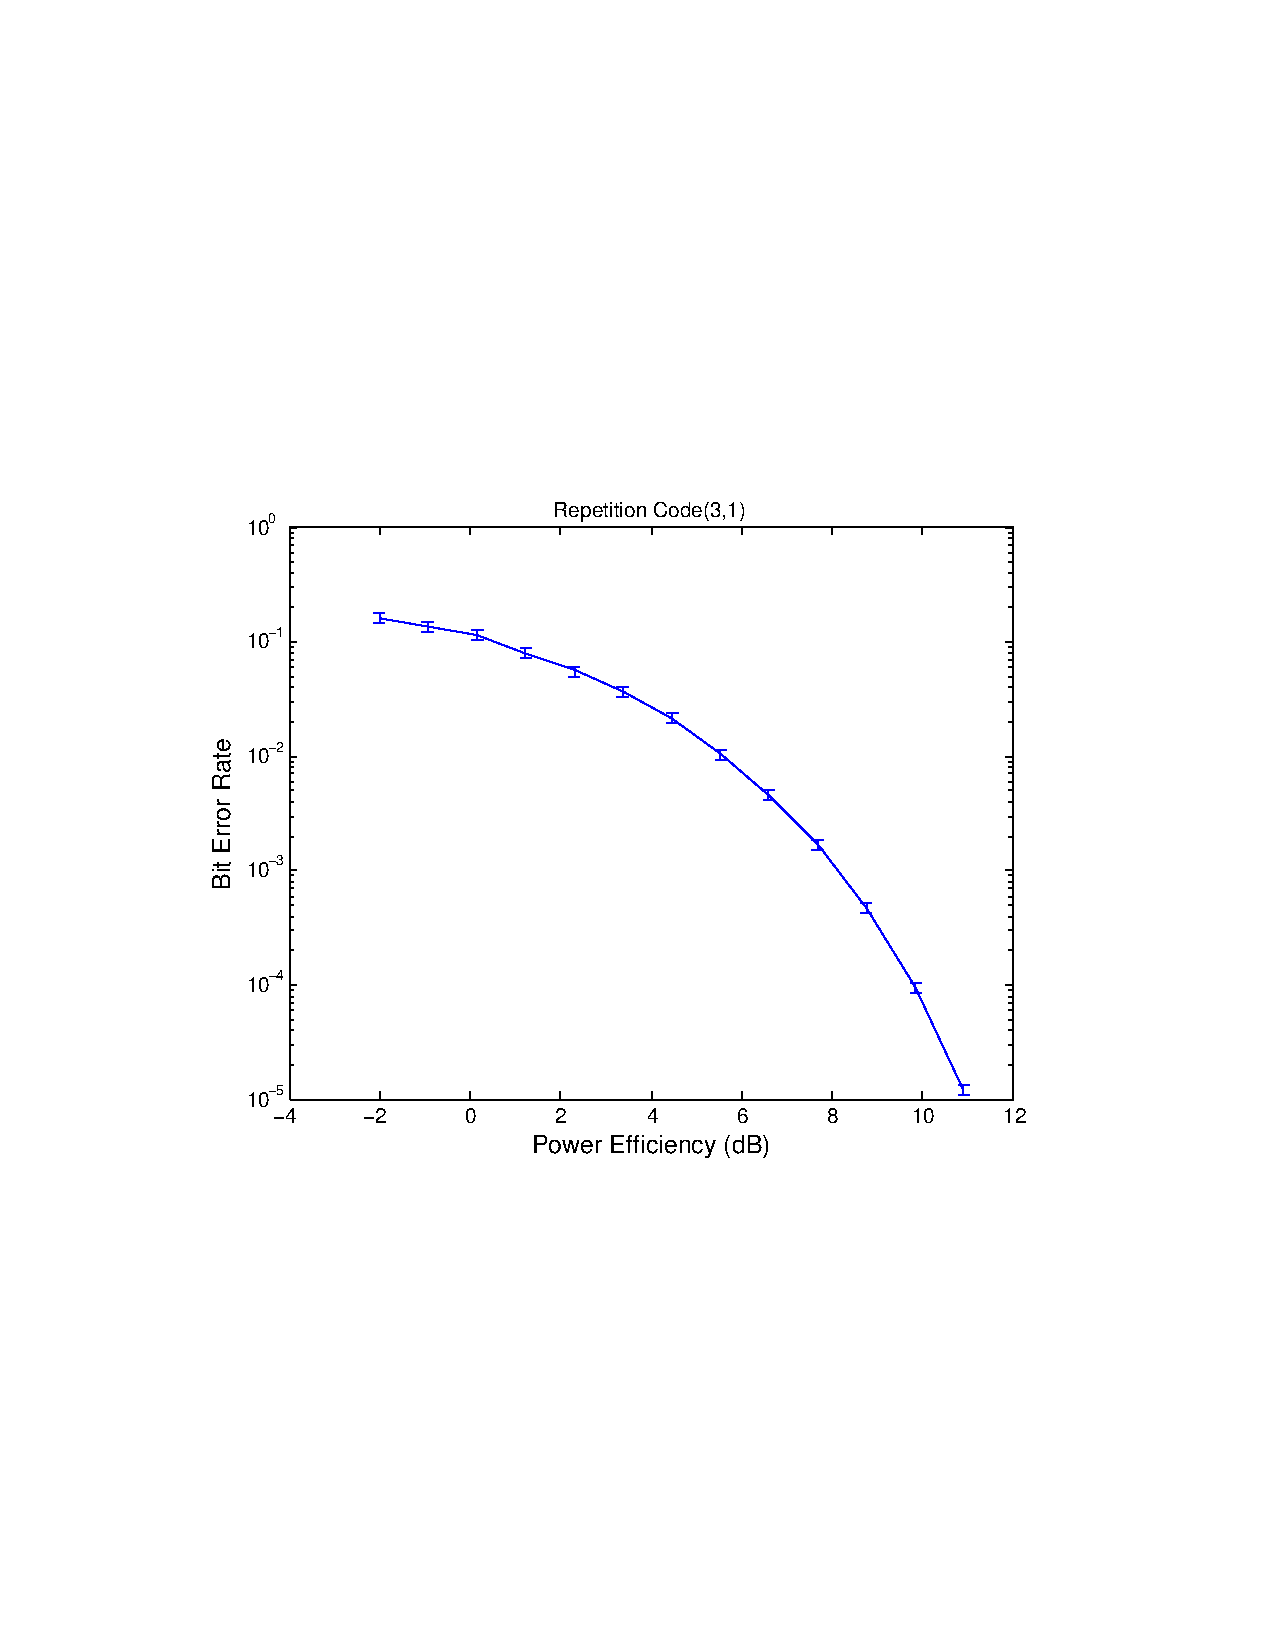
\includegraphics[width=.8\textwidth]{repetition_3_1.pdf}
    \caption{Variation of Bit error rate of Repetition Codes (3,1)}
    \label{rl3}
\end{figure}

\begin{figure}[H]
    \centering
    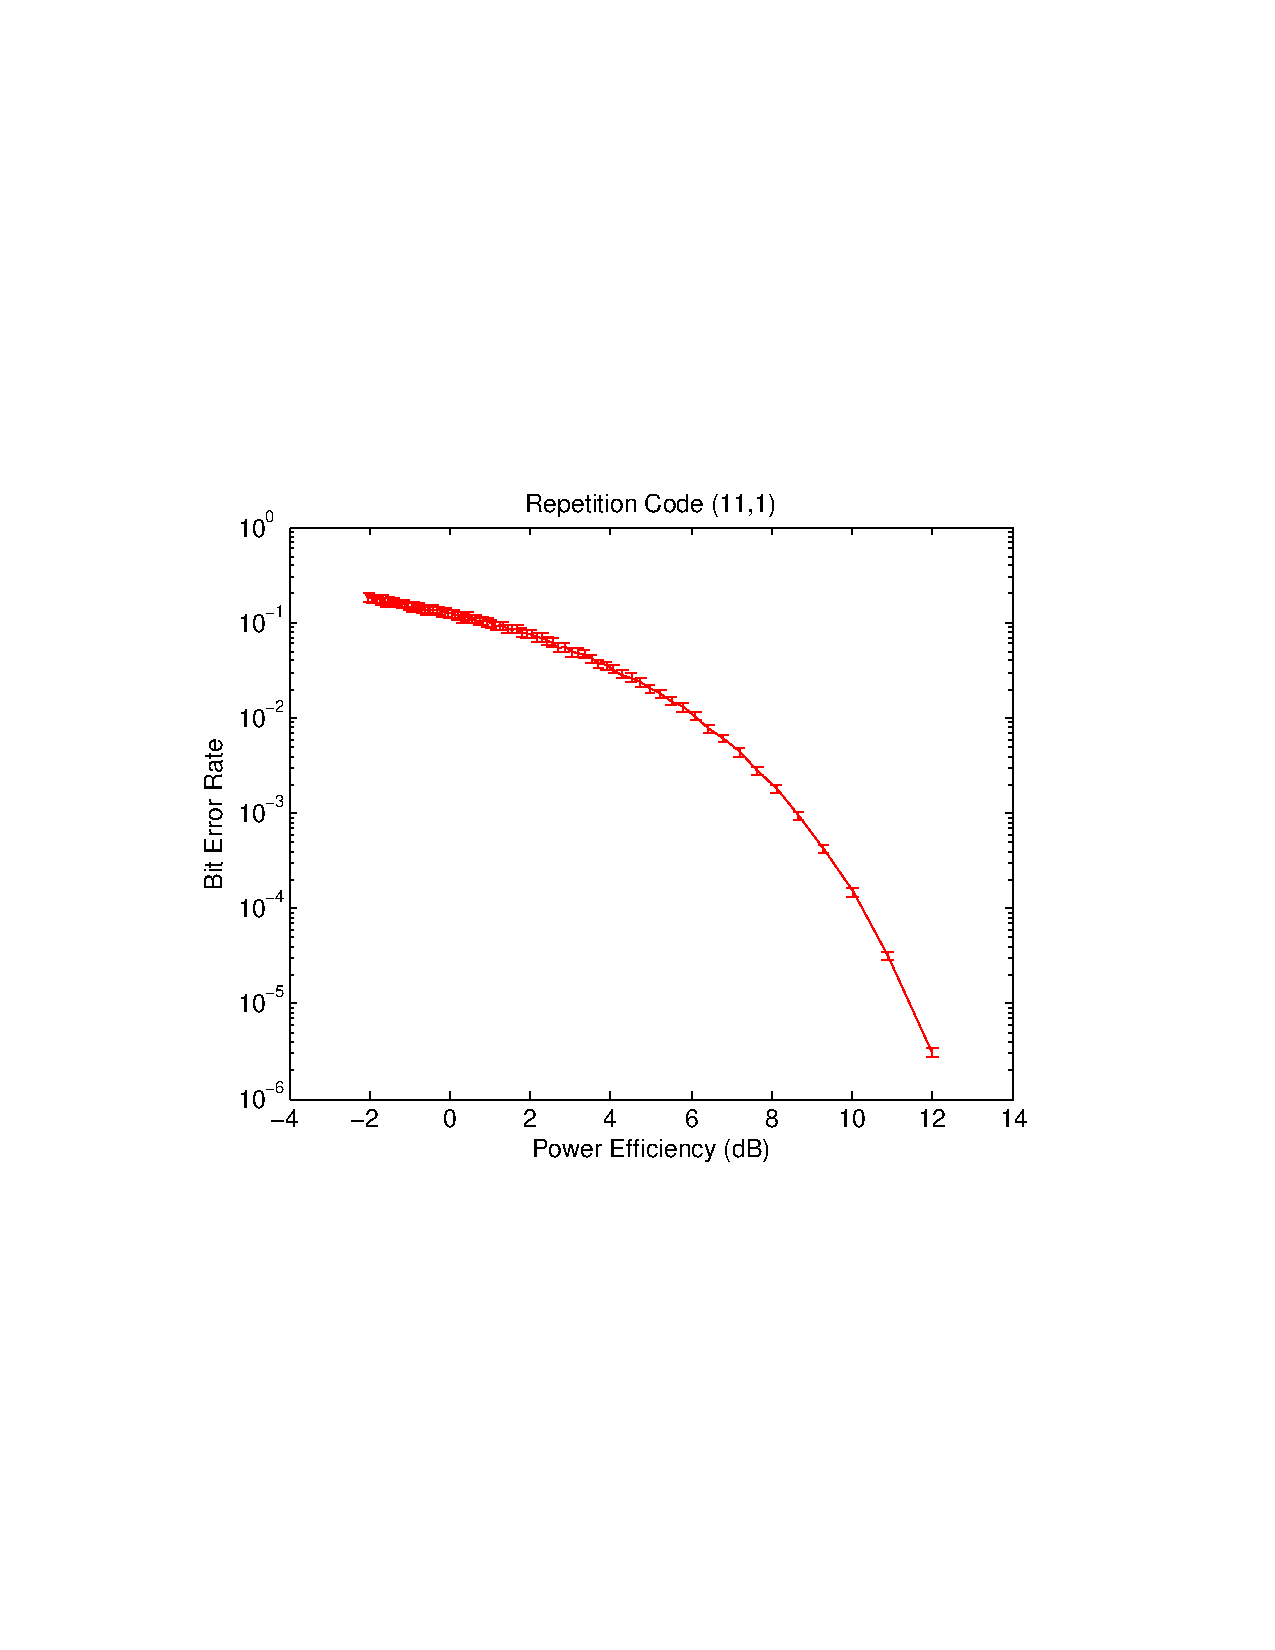
\includegraphics[width=.8\textwidth]{repetition_11_1.pdf}
    \caption{Variation of Bit error rate of Repetition Codes (11,1)}
    \label{rl11}
\end{figure}

\section{Question 4: Hamming Codes}
\subsection{15,11 Hamming Codes}
\begin{figure}[H]
    \centering
    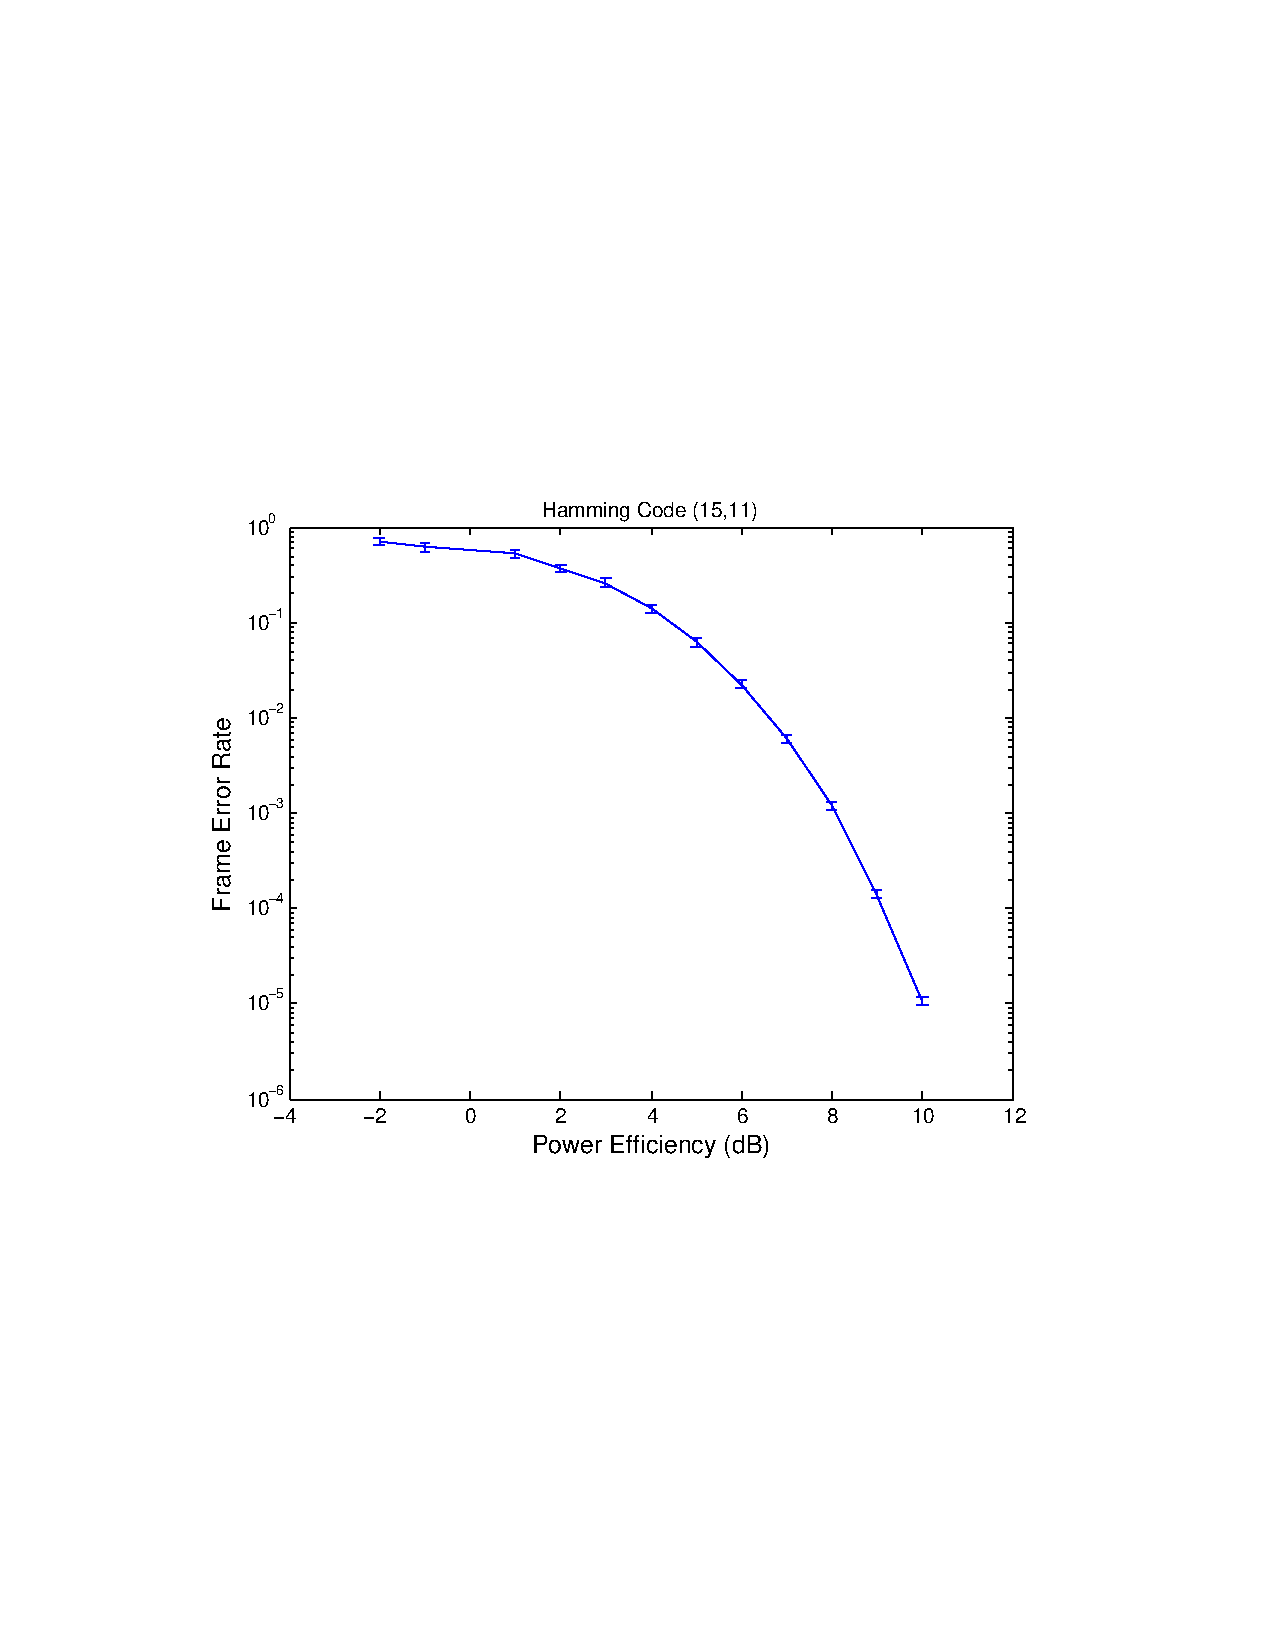
\includegraphics[width=.8\textwidth]{hamming_5_11_incomplete_run_fer.pdf}
    \caption{Variation of Frame error rate of Hamming Codes (15,11)}
    \label{ham_15_11_fer}
\end{figure}

\begin{figure}[H]
    \centering
    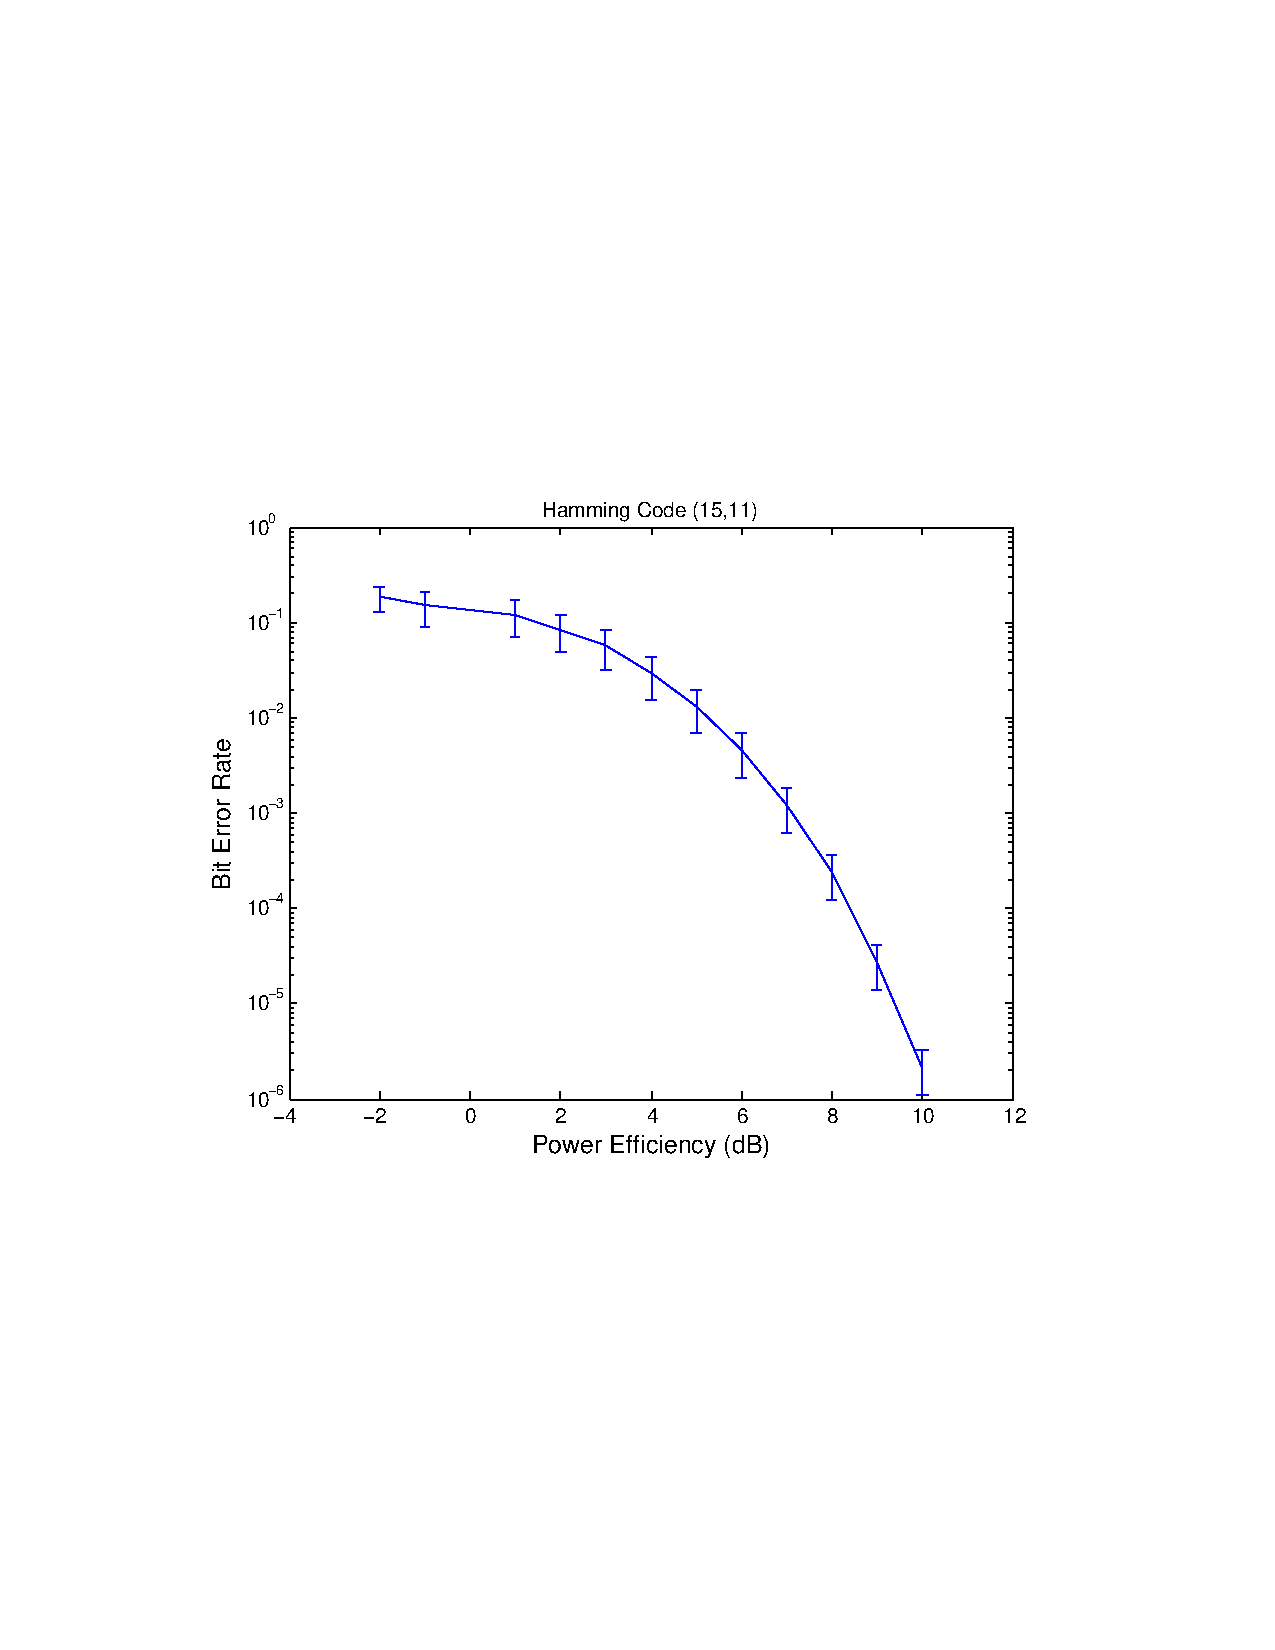
\includegraphics[width=.8\textwidth]{hamming_15_11_incomplete_run_ber.pdf}
    \caption{Variation of Bit error rate of Hamming Codes (15,11)}
    \label{ham_15_11_ber}
\end{figure}


\subsection{3,4 Hamming Codes}

\begin{figure}[H]
    \centering
    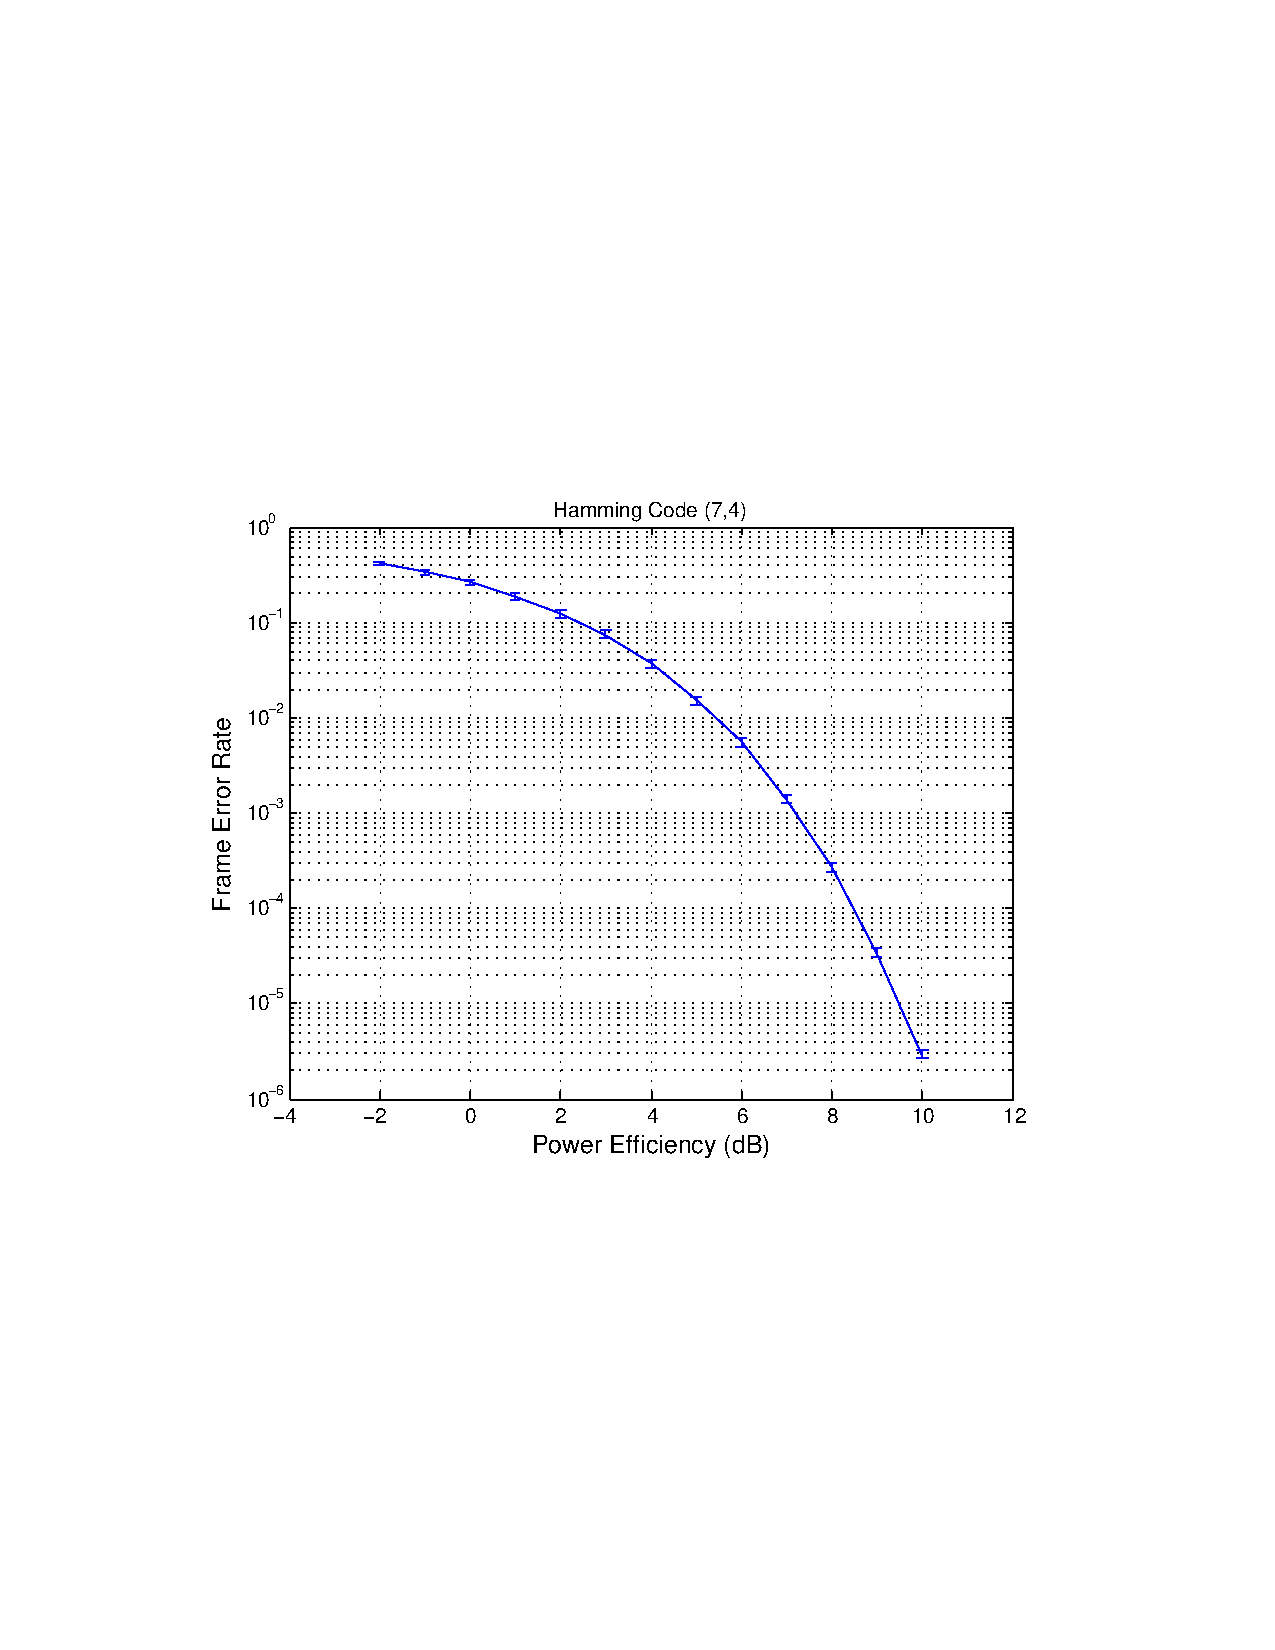
\includegraphics[width=.8\textwidth]{fer_hamming_3_4.pdf}
    \caption{Variation of Frame error rate of Hamming (3,4)}
    \label{f31}
\end{figure}

\begin{figure}[H]
    \centering
    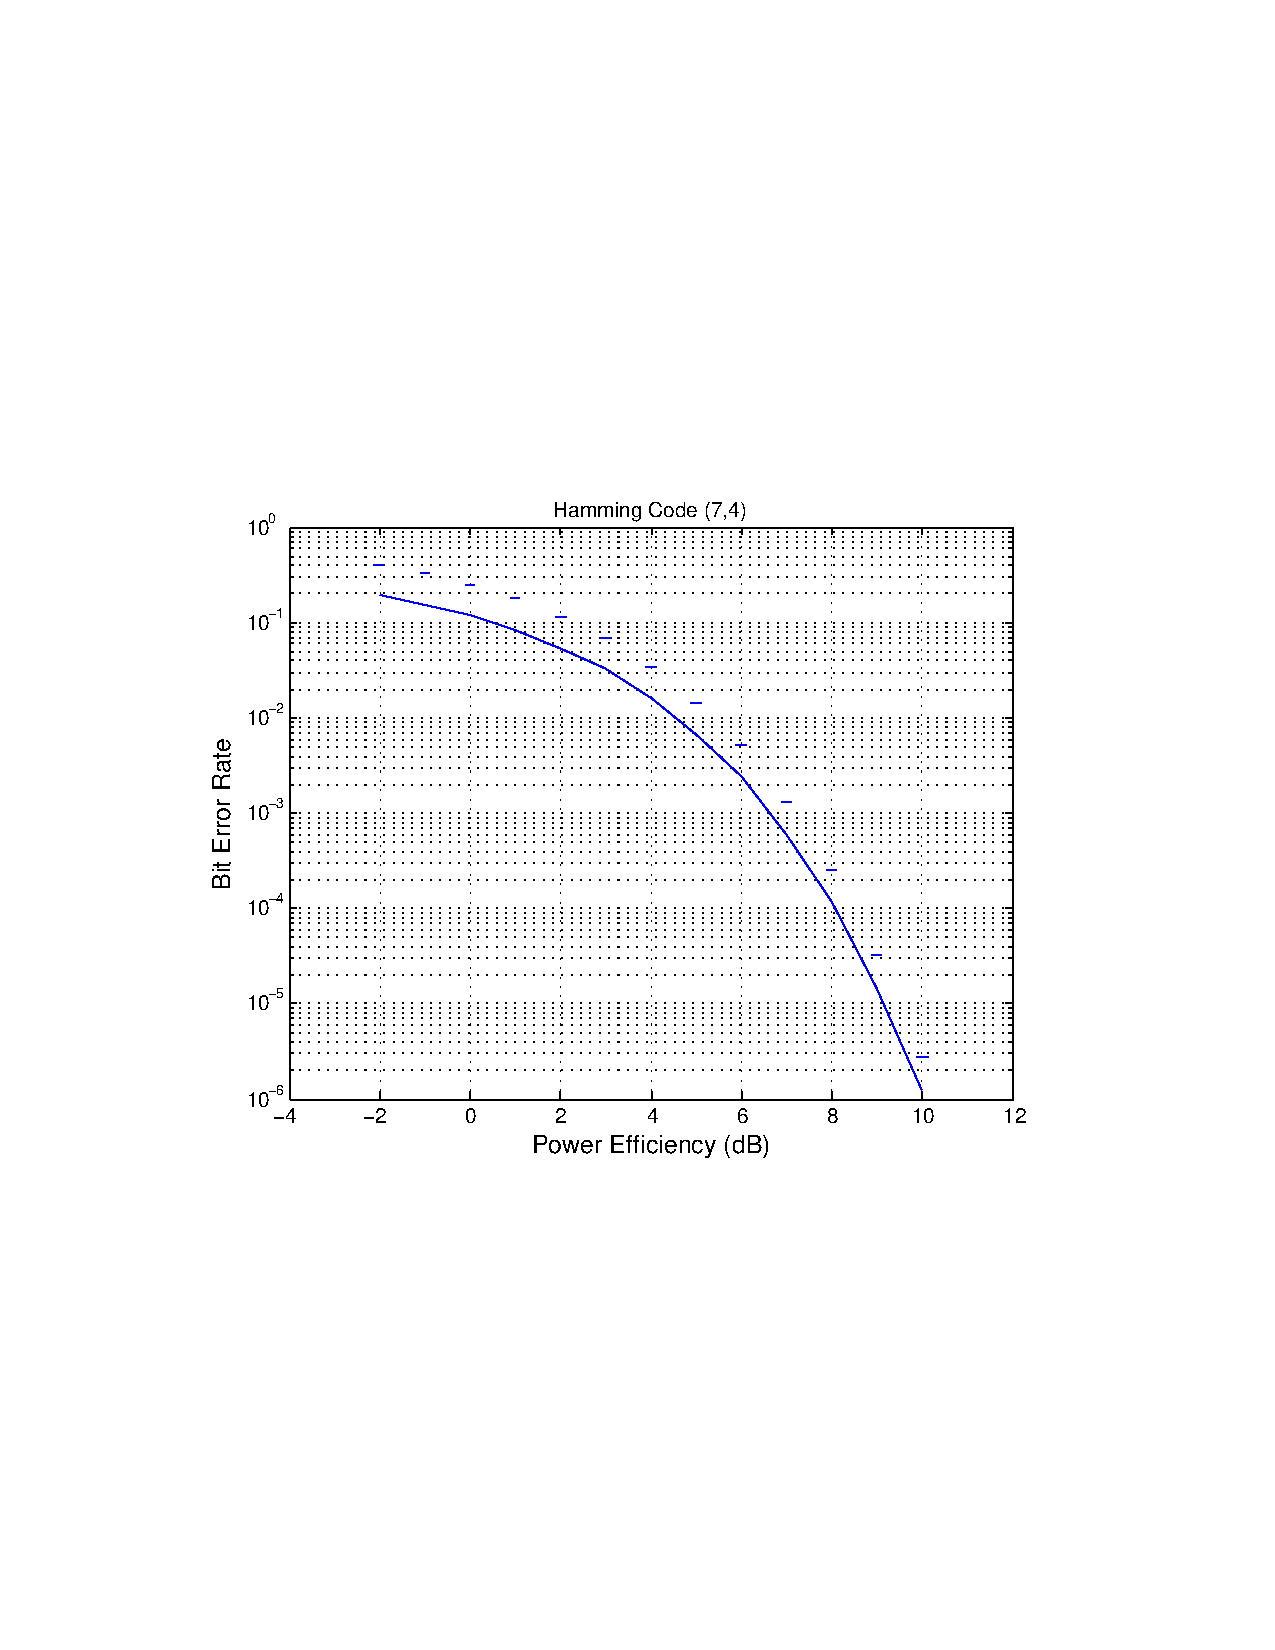
\includegraphics[width=.8\textwidth]{ber_hamming_3_4.pdf}
    \caption{Variation of Bit error rate of Hamming (3,4)}
    \label{h34}
\end{figure}

\subsection{31, 26 Hamming Codes}
\begin{figure}[H]
    \centering
    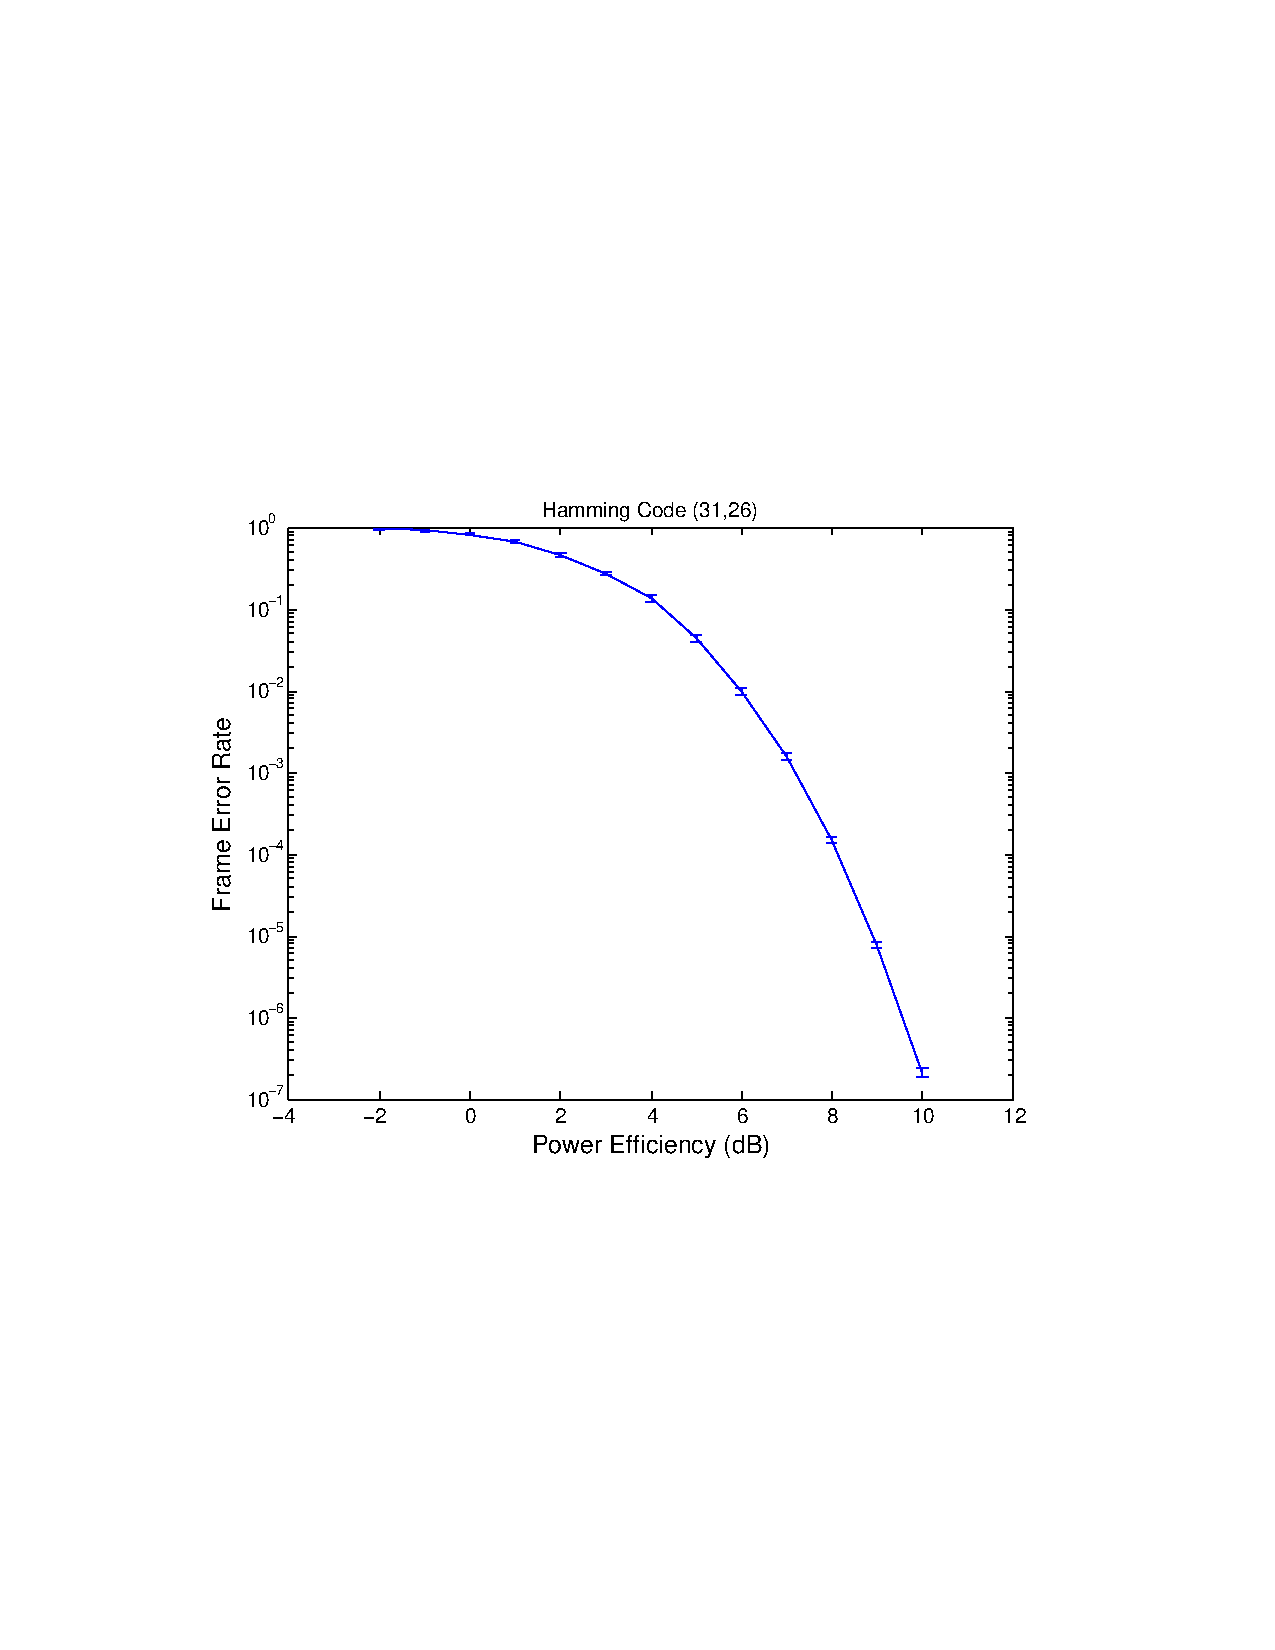
\includegraphics[width=.8\textwidth]{hamming_31_26_fer.pdf}
    \caption{Variation of Frame error rate of Hamming (31,26)}
    \label{h31}
\end{figure}

\begin{figure}
    \centering
    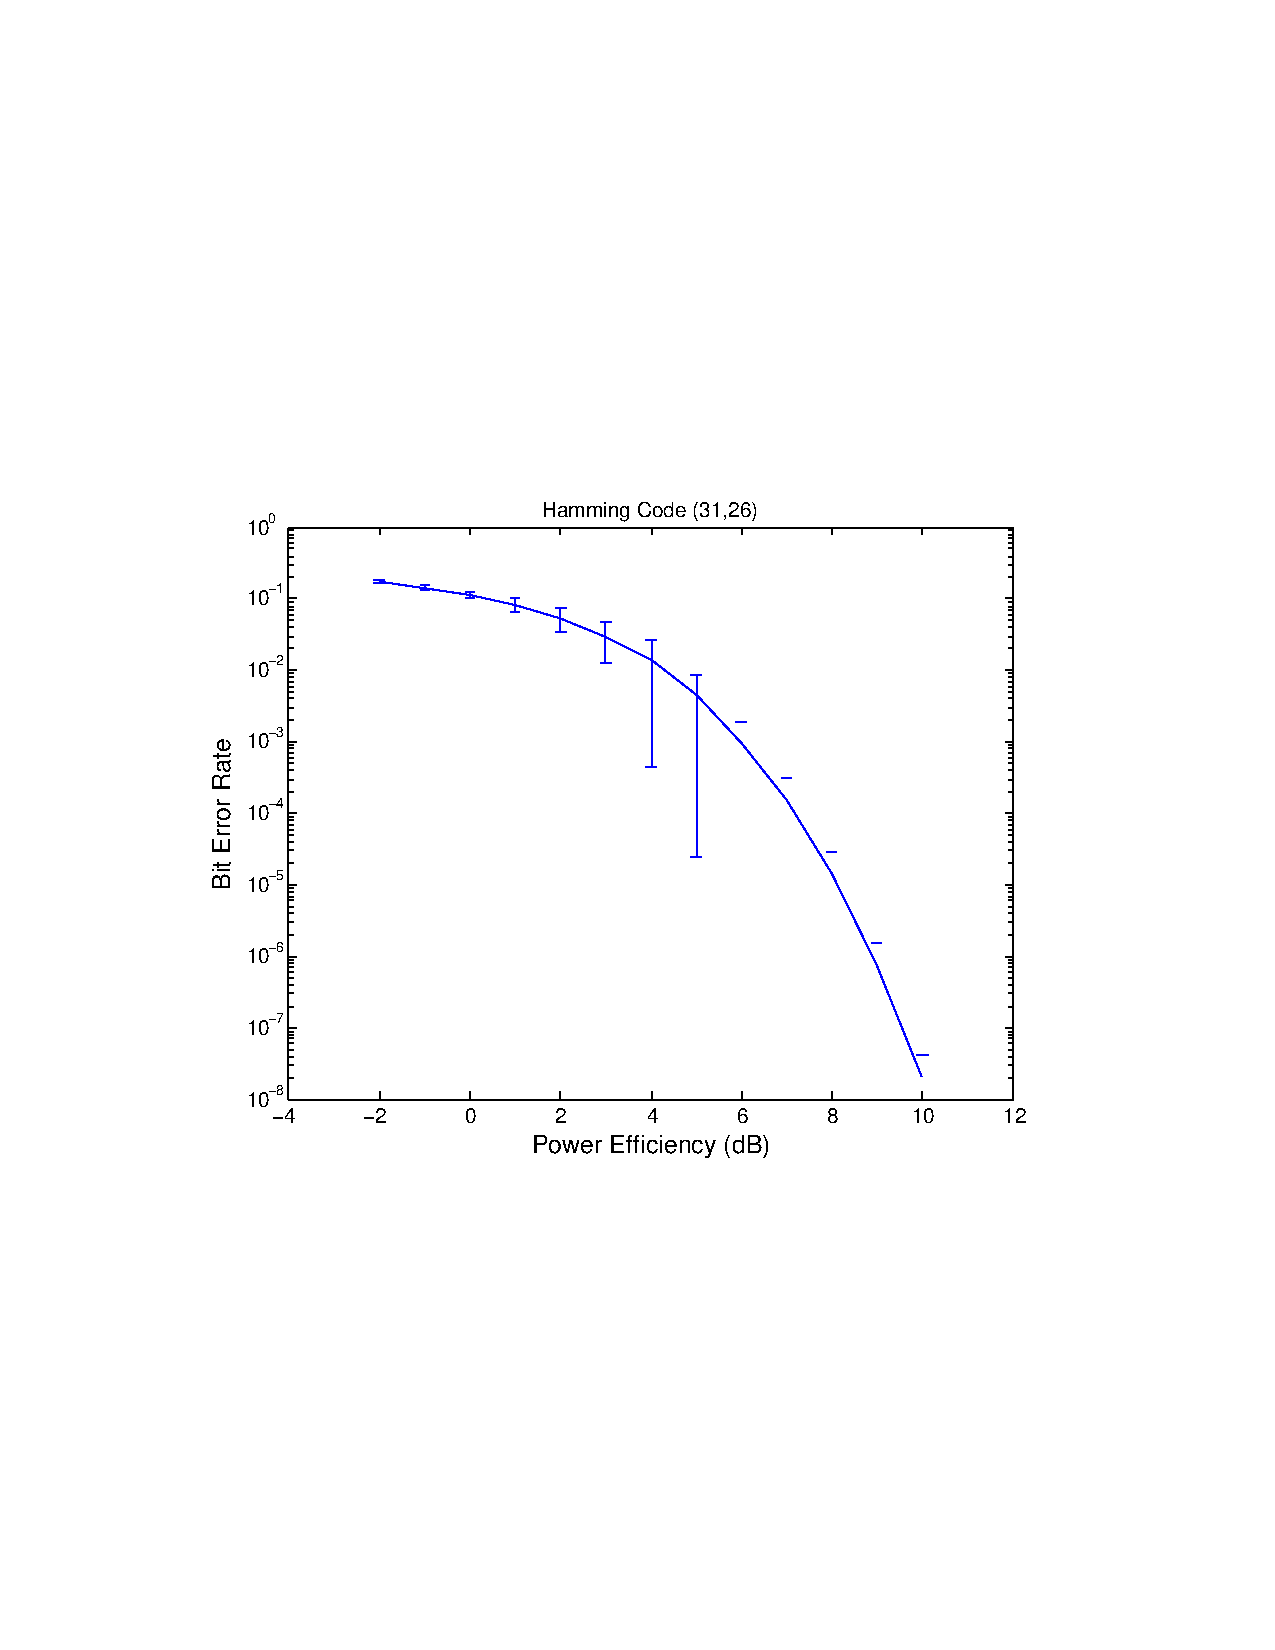
\includegraphics[width=.8\textwidth]{hamming_31_26_ber.pdf}
    \caption{Variation of Bit error rate of Hamming (31,26)}
    \label{b31}
\end{figure}


\section{Question 4: Simplex Code}
\subsection{Syndrome Decoding}

\begin{figure}[H]
    \centering
    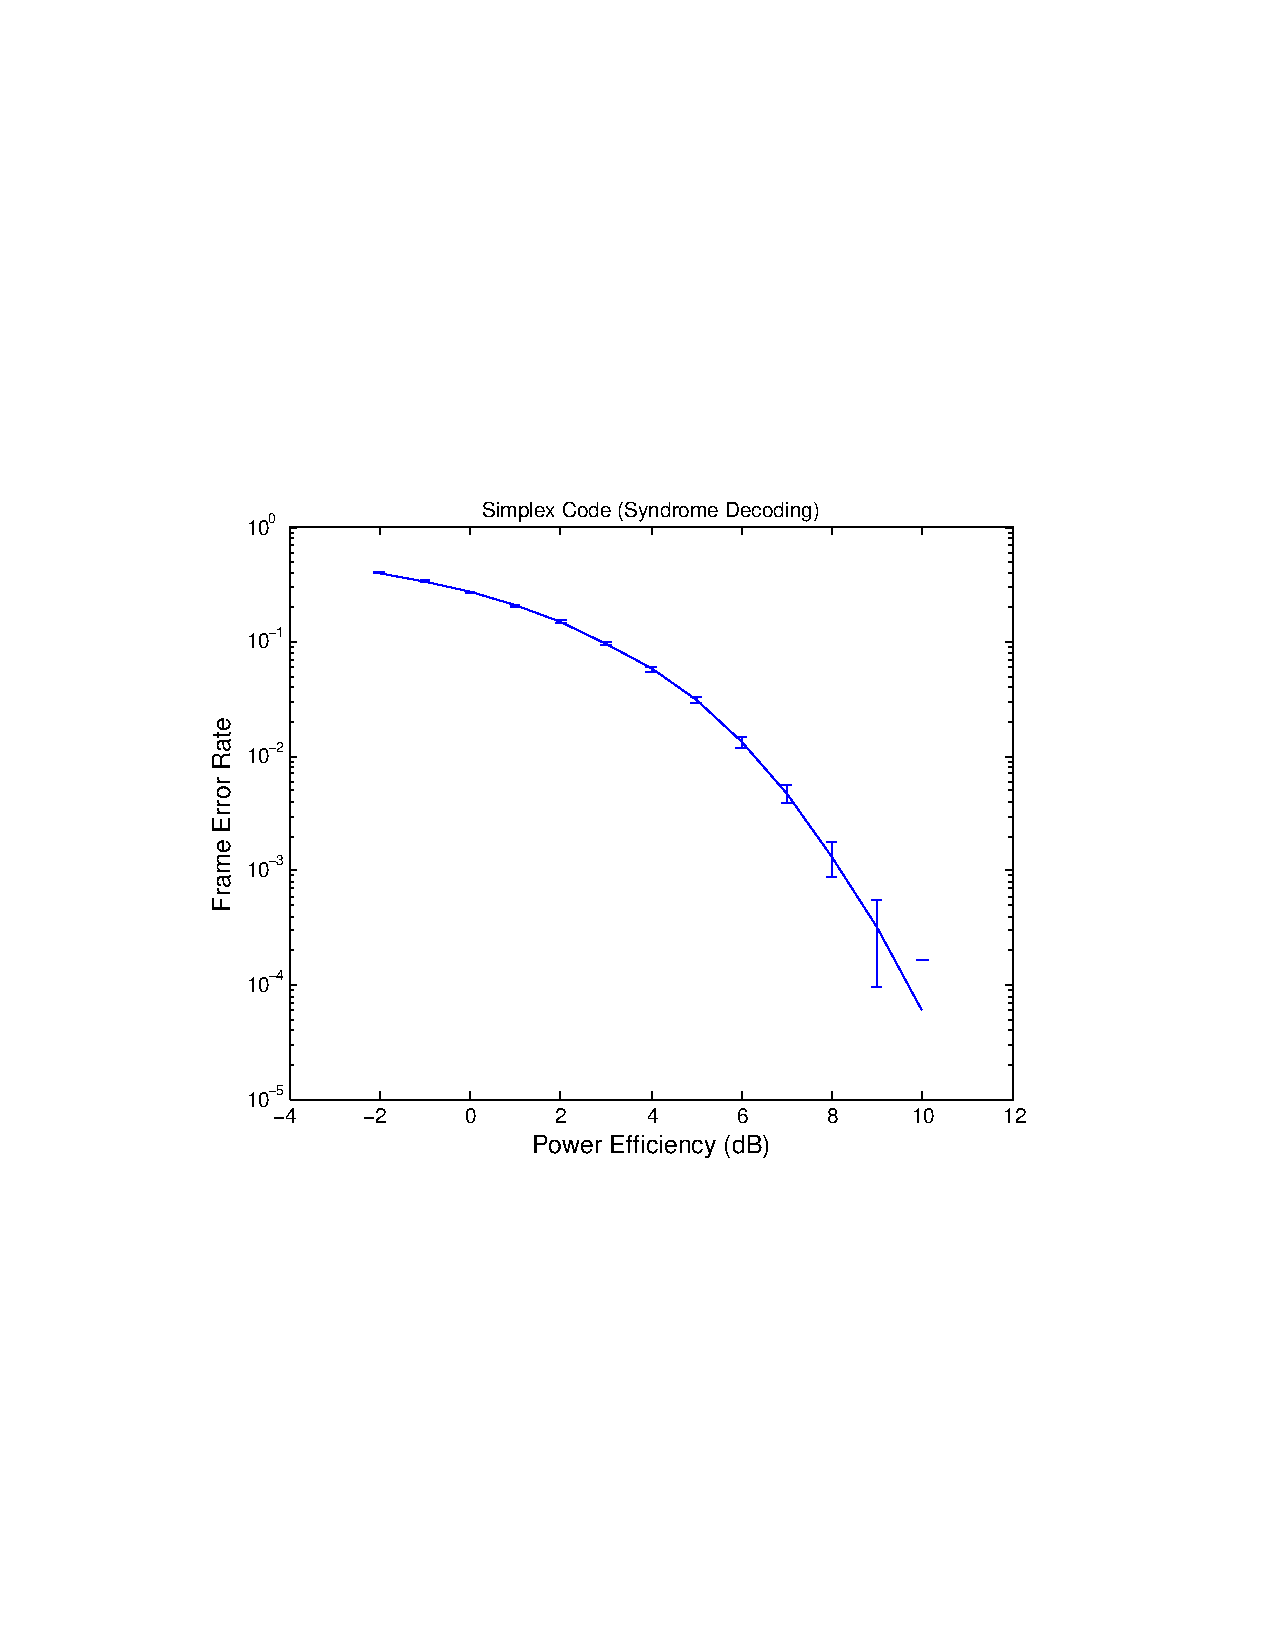
\includegraphics[width=.8\textwidth]{simplex_syndrome_decoding_fer.pdf}
    \caption{Variation of Frame error rate of of Simplex, Syndrome decoding }
    \label{sb2}
\end{figure}

\begin{figure}[H]
    \centering
    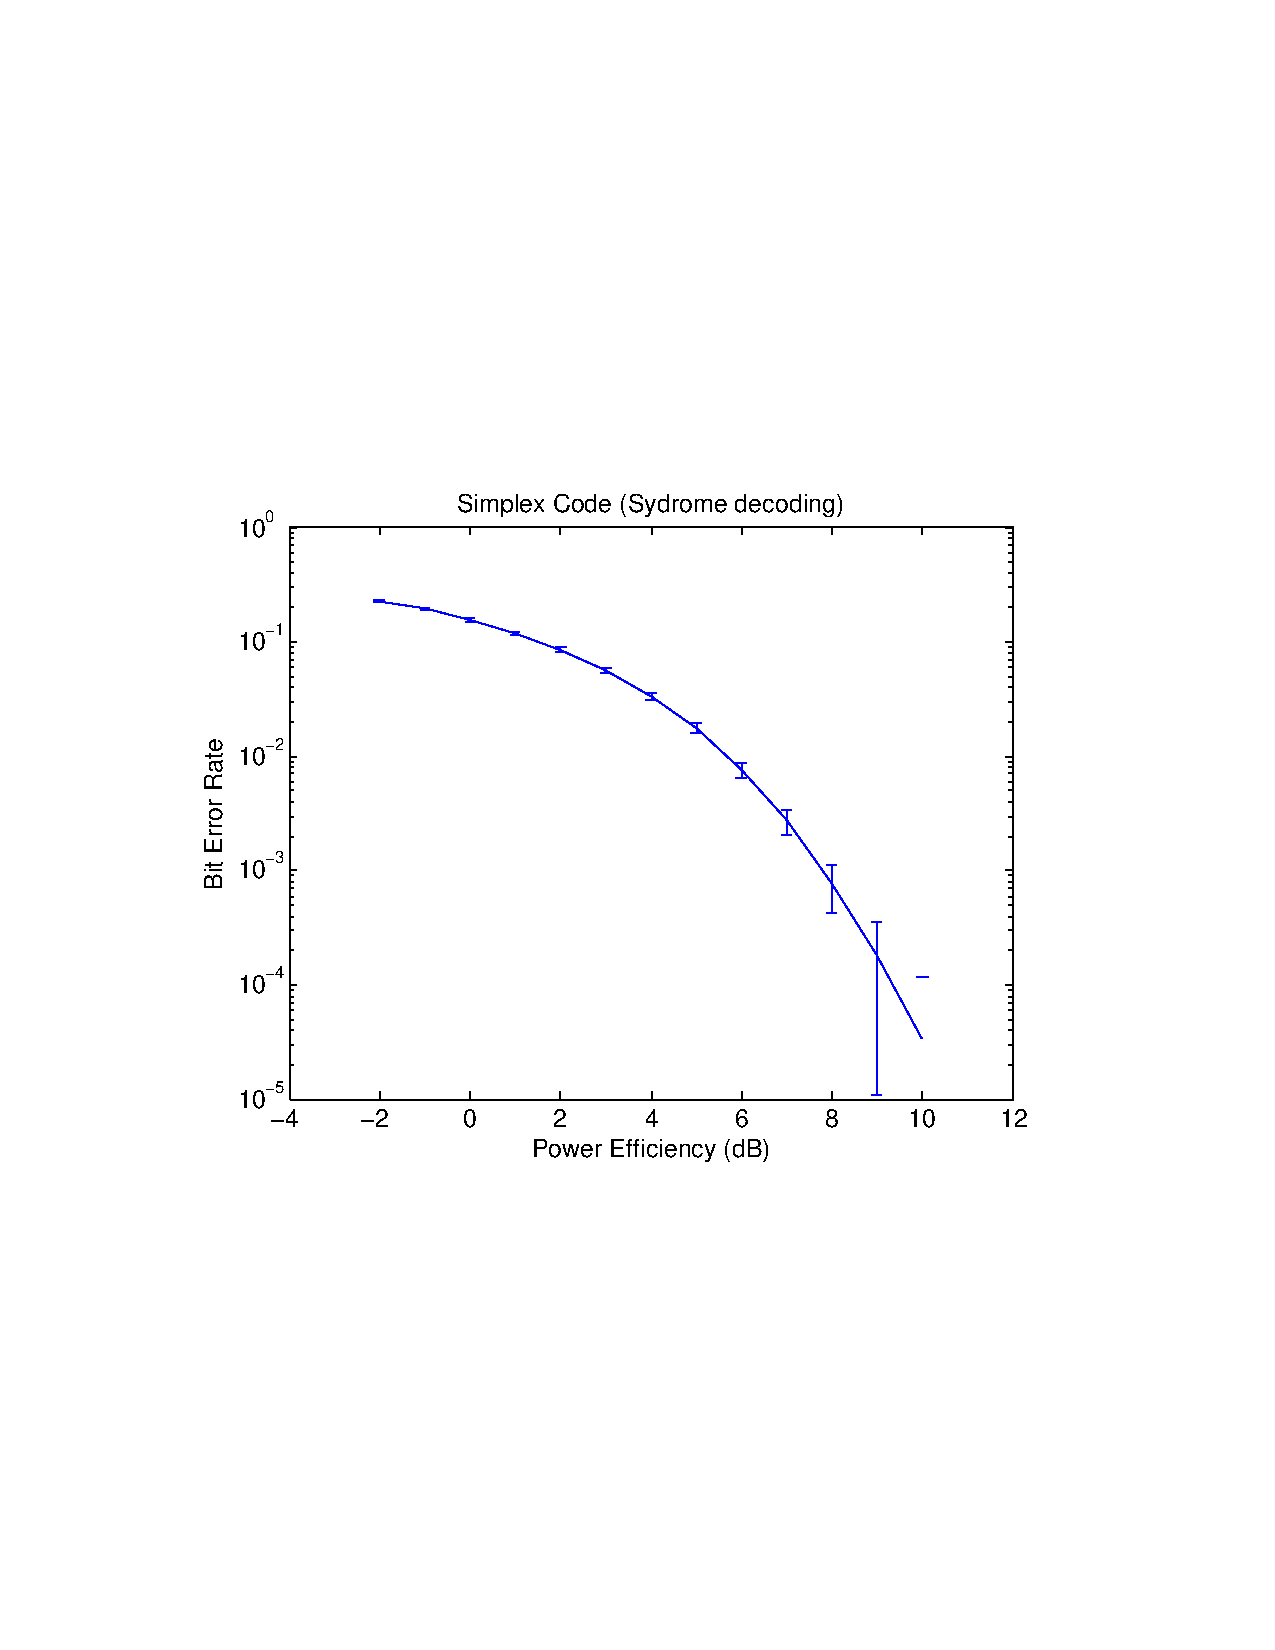
\includegraphics[width=.8\textwidth]{simplex_syndrome_decoding_ber.pdf}
    \caption{Variation of Bit error rate of of Simplex, Syndrome decoding }
    \label{sb1}
\end{figure}

\subsection{Bounded Distance Decoding}
\begin{figure}[H]
    \centering
    \includegraphics[width=.8\textwidth]{.pdf}
    \caption{Variation of Bit error rate of of Simplex, bounded distance decoder}
    \label{sb}
\end{figure}
\begin{figure}[H]
    \centering
    \includegraphics[width=.8\textwidth]{.pdf}
    \caption{Variation of Frame error rate of of Simplex, bounded distance decoder}
    \label{sb}
\end{figure}
\section{Question 5: Golay Code}

\end{document}
